\unfinished{Write method }
The experiments performed is covered in the \textit{jupyter} notebook in the \href{https://github.com/mlRosenquist/au-mlr-computer-vision-and-ml/tree/master/project/notebook.ipynb}{source code}.
\unfinished{Præsenter afsnit}
\unfinished{Source code}
\unfinished{Præsenter sklearn}

\subsection{Dataset}
The dataset is in advance split in training, validation and test sets. The training and validation observations are labeled. The idea is to train the model on the training set and evaluate the performance on the out-of-sample observations from the validation sets.  

\subsection{Preprocesssing}
The dataset contains two types of features - boolean (yes/no) and continous values (numeric). The dataset is not complete, meaning some observations are missing values in certain features. To overcome this the mean value is used for the numeric features and the most popular for the boolean features. As the features are in different units it is important to scale the data. Without scaling certain features might dominate the other features. This is specially the case for SVC, because it tries to maximize the distance between the support vectors and the hyperplane. \textit{sklearn} have different options for scaling; StandardScaler, MinMaxScaler and RobustScaler. The MinMaxScaler with default settings will suffice with a scaling of each feature individually between 0 and 1 \todo{cite}.        

\subsection{Model training}
Tuning the model to perform as desired is not a trivial task and it is highly dependent on the use case. Initially, there is several questions to be answered such as: How do we train the model? Do we use the raw training data? Are we to use sampling methods? How do we test different model parameters? Which metrics are used to train/evaluate the model? Answering these differently will lead to very diverse models. Due to lack of experience, this section will cover a trial and error approach. Firstly, a model is trained with default parameters. Then we look into tuning the model in various ways. The different models are concurrently evaluated. \\

\textit{sklearn}'s SVC implementation is used to build the model. Initially we try the model with the default parameters: 
\begin{itemize}
  \item Regularization parameter (C): 1
  \item Kernel: Radial Basis Function (rbf)
\end{itemize}

\noindent The model is trained and evaluated. The evaluation on the validation set can be seen on Figure \ref{fig:results_default}.

\begin{figure}[H]
  \centering
  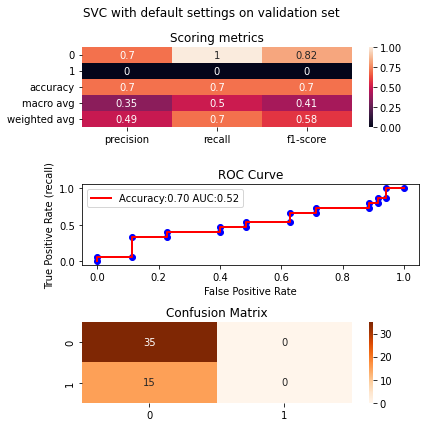
\includegraphics[width=0.4\textwidth]{../project/images/results_default-svc.png}
  \caption{Performance of SVC model with default parameters}
  \label{fig:results_default}
\end{figure}
It is seen that the model scores well in terms of precision, recall and f1-score on class \textit{0}. However, as seen in the confusion matrix this is due to the model classifying all observations to class \textit{0}. This is due to the concerns introduced earlier regarding imbalanced data. As a measure, we balance the weights of each class. This is done by settings the model's \textit{class\_weight} parameter to \textit{balanced}. \textit{class\_weights} can be defined explicitly or have \textit{sklearn} calculate them by the proportions. The validation performance can be seen on Figure \ref{fig:results_default_balanced}.

\begin{figure}[H]
  \centering
  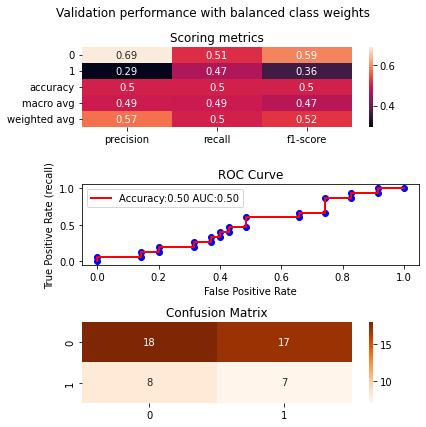
\includegraphics[width=0.4\textwidth]{../project/images/results_default_balanced-svc.png}
  \caption{Performance of SVC model with balanced class weights}
  \label{fig:results_default_balanced}
\end{figure}

The update in class weights clearly makes the model predict more observations to class 1. This leads to better scoring of class 1, but many false positives are introduced as a consequence. To mitigate these, we try to tune other parameters of the model. We do this with \textit{sklearn} \textit{GridSearchCV} implementation. Here we can define a grid of parameters and train models with each combination of the parameters. Additionally, we utilize stratified cross validation with 5 folds. Being stratified means that we have the same class ratio across all folds. We define a grid with different options for the regularization parameter, C. The performance of the models on each folds can be seen on Figure \ref{fig:results_gridcv_balanced_C}.     

\begin{figure}[H]
  \centering
  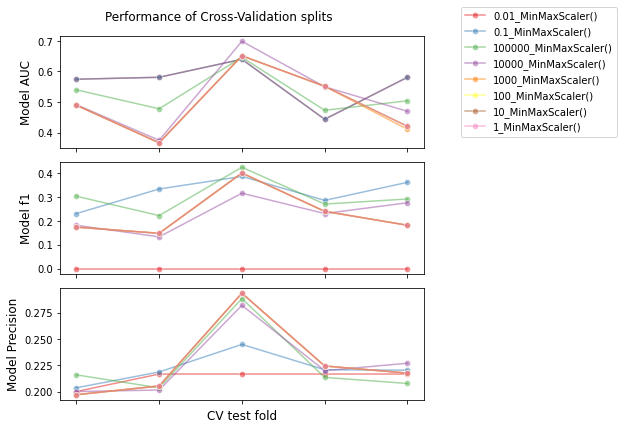
\includegraphics[width=0.5\textwidth]{../project/images/results_gridcv_balanced-C.png}
  \caption{Cross-validation performance of SVC model with different C values}
  \label{fig:results_gridcv_balanced_C}
\end{figure}
There are eight different $C$ values. However, less are showed on the plots. This is due to models performing similarly with nearby values. Looking at the different metrics; AUC, f1, precision, it can be seen that different C values affect the models. Additionally, models performing well at one metric might not succeed according to another metric. The best model is selected according to the average precision metric. The validation performance is evaluated. On figure \ref{fig:results_gridcv_balanced_C_metrics} it shows, that we have less false positives and true positives.   
\begin{figure}[H]
  \centering
  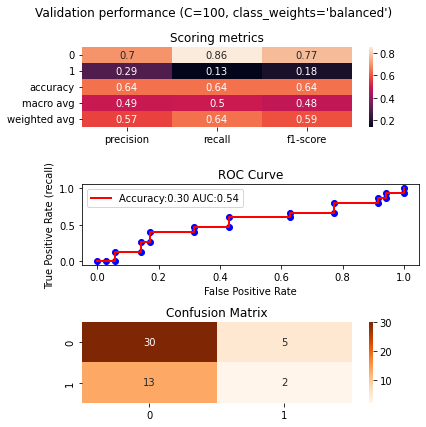
\includegraphics[width=0.4\textwidth]{../project/images/results_gridcv_balanced-C_metrics.png}
  \caption{Performance of best model looking at \textit{C}}
  \label{fig:results_gridcv_balanced_C_metrics}
\end{figure}

There are still many misclassified observations. The next step that we will is feature selection. We will utilize \textit{SelectKBest} with \textit{chi2} as selection method. The selection step is included in the grid search of the best set of parameters. We try with a range of \textit{k} features. The best model according to precision ends up being, \textit{k=21, C=100}. The performance of this model can be seen on Figure \ref{fig:results_gridcv_balanced_C_selKBest}.

\begin{figure}[H]
  \centering
  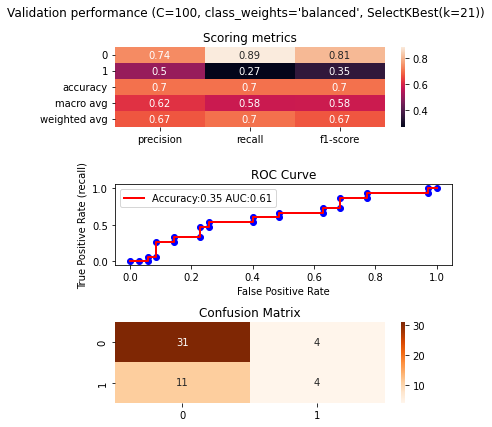
\includegraphics[width=0.4\textwidth]{../project/images/results_gridcv_balanced-C-selectKBest.png}
  \caption{Performance of best model looking at \textit{C} and SelectKBest}
  \label{fig:results_gridcv_balanced_C_selKBest}
\end{figure}

The model seems to identify less false positives while classifying more true positives. Hence, selecting 21 features seems to be positive for the model. Next we will try different kernels of the SVC model. It showed that the default kernel that was utilized already, Radial Basis Functions, is the best performer according to precision.     



